\documentclass[12pt]{article}
\usepackage[brazil]{babel}
\usepackage{graphicx}
\usepackage{mathtools}
\usepackage{float} 
\usepackage{xcolor}
\usepackage{amsmath, amssymb, bm}


\usepackage{array}
\usepackage{booktabs}



% margenes
\usepackage[a4paper,left=3cm,right=3cm,top=3cm]{geometry}

%opening
\title{}
\author{}

\begin{document}

\begin{center}
	{\tiny {\normalsize {\large \textbf{Convecção}\\ Lista de exercicios 2\\
	
	\textbf{Cristian Herledy Lopez Lara}}}}
\end{center}

\subsection*{Exercício 2,19 livro texto}


\textbf{Considerando a análise de transferência de calor do problema 2.18 e levando em conta que L é longo o suficiente para que o fluxo de calor qb não dependa de L, Determinar: A) Se b aumenta a uma taxa de duas vezes, por qual fator qb aumentará? B) Calcule a razão $q_{B,w}/q_{B,a}$} \\



\textbf{Informações de entrada} 

Do problema 2,18:

\begin{equation}
	\begin{aligned}
		q_{B} = (T_{B} - T_{\infty})(hpkA)^{\frac{1}{2}}\ tanh\left[L(\frac{hp}{kA})^{\frac{1}{2}}\right] 
	\end{aligned}
\end{equation}

\begin{equation}
	\begin{aligned}
		\frac{hb}{k_{f}}=0,664Pr^{\frac{1}{3}}\left(\frac{U_{\infty }b}{\nu} \right)^{\frac{1}{2}} 
	\end{aligned}
\end{equation}

\begin{figure}[H]
	\centering
	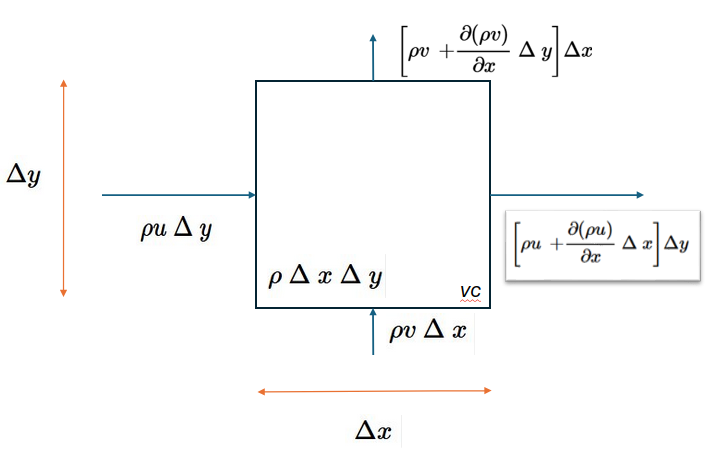
\includegraphics[width=.65\textwidth]{Figures/1_1}
	\caption{Transferência de calor em aleta com fluxo laminar paralelo a b}
\end{figure}

Como $x\approx L$, supõe-se que seja longo o suficiente para não influenciar o comportamento de $q_{B}$, então $tanhL\rightarrow1$ na equaçao (1)

\begin{equation}
	\begin{aligned}
		q_{B} = (T_{B} - T_{\infty})(hpkA)^{\frac{1}{2}}\  
	\end{aligned}
\end{equation}

Considerando que $p=2b$, $A=bt$ e calculando h de (2):



\begin{equation}
	\begin{aligned}
		q_{B} = (T_{B} - T_{\infty})\left(\frac{0,664Pr^{\frac{1}{3}}k_{f}kbt2b}{b}\left(\frac{U_{\infty}b}{\nu}\right)^{\frac{1}{2}}\right)^{\frac{1}{2}}\  
	\end{aligned}
\end{equation}
\textbf{Item A}

A partir da equaçao (4), a relação entre qb e b é encontrada 

\begin{equation}
	\begin{aligned}
		q_{B} = (T_{B} - T_{\infty})\left(1,328Pr^{\frac{1}{3}}k_{f}kt\left(\frac{U_{\infty}}{\nu}\right)^{\frac{1}{2}}\right)^{\frac{1}{2}} b^{\frac{3}{4}} 
	\end{aligned}
\end{equation}

Por tanto, $q_{B}$ é proporcional a b na forma

\begin{equation}
	\begin{aligned}
		q_{B} \sim b^{\frac{\scriptstyle 3}{\scriptstyle 4}}
	\end{aligned}
\end{equation}
\begin{equation}
	\begin{aligned}
		q_{B} \sim 2^{\frac{\scriptstyle 3}{\scriptstyle 4}} = 1,68
	\end{aligned}
\end{equation}

Quando a altura da aleta é \textbf{dobrada}, a taxa de transferência de calor \textbf{aumenta em 68\%}
\\

\textbf{Item B}

Os raios podem ser calculados substituindo as propriedades de cada fluido na equação (5)

\begin{equation}
	\begin{aligned}
		\frac{q_{B,w}}{q_{B,a}} = \frac{(T_{B} - T_{\infty})\left(1,328Pr^{\frac{1}{3}}_{w}k_{w}kt\left(\frac{U_{\infty}}{\nu_{w}}\right)^{\frac{1}{2}}\right)^{\frac{1}{2}} b^{\frac{3}{4}} }{(T_{B} - T_{\infty})\left(1,328Pr^{\frac{1}{3}}_{a}k_{a}kt\left(\frac{U_{\infty}}{\nu_{a}}\right)^{\frac{1}{2}}\right)^{\frac{1}{2}} b^{\frac{3}{4}} }
	\end{aligned}
\end{equation}

Propriedades do escoamento como a velocidade, temperatura e volume, são constantes para cada caso. A razões total pode ser calculada a partir das razões das propriedades do fluido.

\begin{equation}
	\begin{aligned}
		\frac{q_{B,w}}{q_{B,a}} = \frac{\left(Pr^{\frac{1}{3}}_{w}k_{w} \nu^{-\frac{1}{2}}_{w}\right)^{\frac{1}{2}}  }{\left(Pr^{\frac{1}{3}}_{a}k_{a}\nu^{-\frac{1}{2}}_{a}\right)^{\frac{1}{2}}  }\ \ = \ \ \left( \frac{Pr_{w}}{Pr_{a}}\right)^{\frac{1}{6}} \left( \frac{\nu_{a}}{\nu_{w}}\right)^{\frac{1}{4}} \left( \frac{k_{a}}{k_{w}}\right)^{\frac{1}{2}}
	\end{aligned}
\end{equation}

\begin{equation}
	\begin{aligned}
		 \left( \frac{7}{0,72}\right)^{\frac{1}{6}} \left( {\frac{1}{0,07}}\right)^{\frac{1}{4}} \left( 23\right)^{\frac{1}{2}} = 13,5
	\end{aligned}
\end{equation}

\end{document}





